\documentclass[twocolumn]{article}

\usepackage[utf8]{inputenc}
\usepackage[margin=0.65in]{geometry}
\usepackage{authblk}
\usepackage{amsmath}
\usepackage{amssymb}
\usepackage{booktabs}
\usepackage{textcomp}
\usepackage{gensymb}
\usepackage{xcolor}
\usepackage{float}
\usepackage{tikz}
\usetikzlibrary{arrows.meta, positioning, fit, backgrounds}
\usepackage{hyperref}

% The 1e (One Euro) filter is conventionally written with a euro sign.
\providecommand{\euro}{\texteuro}

\setlength{\columnsep}{20pt}

\definecolor{blkfill}{HTML}{EEF2F7}
\definecolor{blkline}{HTML}{4A6784}
\definecolor{accfill}{HTML}{FDF1E3}
\definecolor{accline}{HTML}{B5762A}
\hypersetup{colorlinks=true, urlcolor=blkline, linkcolor=black, citecolor=black}
\tikzset{
  blk/.style  = {draw=blkline, fill=blkfill, rounded corners=2pt, align=center,
                 font=\scriptsize, inner sep=3pt, minimum height=7.5mm},
  acc/.style  = {blk, draw=accline, fill=accfill},
  flow/.style = {-{Stealth[length=4pt]}, draw=blkline, thick},
  ret/.style  = {-{Stealth[length=4pt]}, draw=accline, thick, dashed},
  lbl/.style  = {font=\scriptsize\itshape, inner sep=2pt}
}

\usepackage[backend=biber, style=numeric-comp, sorting=none,
            maxbibnames=4, giveninits=true]{biblatex}
\addbibresource{references.bib}

\title{\vspace{-1em}Pose Imitation of Human Motion by a Simulated Humanoid Robot:\\
\large Metric-3D Perception, Whole-Body Retargeting and Balance-Supervised Locomotion}

\author[1]{Salih Keceli}
\author[1]{Tarik Billa}
\author[1]{Niti Shivang Trivedi}
\author[1]{Shantanu Shende}
\author[1]{Sai Radhika Mitta}
\author[1]{Amreen Fatima}

\affil[1]{Department of Information Technology, Electrical Engineering and Mechatronics (IEM)\\
THM University of Applied Sciences, Friedberg, Germany}

\date{September 2026}

\begin{document}
\twocolumn[
\begin{@twocolumnfalse}

\maketitle

\begin{abstract}
\noindent
We present a markerless visual teleoperation system in which a simulated NAO~H25 humanoid
imitates a human recorded by a single RGB camera. Absolute metric 3D landmarks are estimated
with MeTRAbs on a GPU, streamed over UDP, and retargeted on the robot side into whole-body
joint commands under continuous balance supervision. Three decisions distinguish the design
from direct joint copying. Retargeting is a closed-form swing-twist decomposition in a
per-frame torso-local basis, making the mapping invariant to the subject's heading. The twelve
leg joints are owned by exactly one of four control layers on every simulation step, so two
commanders can never contend for one actuator. Since a monocular camera cannot observe the
robot's centre of mass, the camera supplies only the desired leg pose while the robot's
forward-kinematics mass model decides how much is executable, with authority granted by the
pose's symmetry rather than its magnitude. Locomotion plays pre-balanced motion clips entered
through a travel-synchronised ramp and, where a clip contains a limit cycle, rewound at a seam
measured at $0.0000$~rad, raising sustained walking speed from $0.036$ to $0.073$~m/s. Turning
is aimed rather than chained: pairing each certified stopping keyframe with the yaw delivered
by then converts one coarse clip into a ladder of $104$ reachable angles, cutting a
$90\degree$ turn from three clips to one and the mean residual heading error from $21.6\degree$
to $3.9\degree$. The implementation is $28{,}496$ lines of Python, of which $9{,}535$ are tests,
all $575$ passing. We report perception timings measured at $16.0$~FPS over $31{,}243$ recorded
frames, locomotion outcomes derived from clip kinematics, an analysis of $8{,}153$~s of
instrumented simulation that exposes a session-wide locomotion kill switch, and a Webots
\texttt{InertialUnit} axis-masking defect that halves the reported torso pitch.
\end{abstract}
\vspace{1em}
\end{@twocolumnfalse}
]

%%%%%%%%%%%%%%%%%%%%%%%%%%%%%%%%%%%%%%%%%%%%%%%%%%%%%%%%%%%%%%%%%%%%%%%%%%%%%%
\section{Introduction}
%%%%%%%%%%%%%%%%%%%%%%%%%%%%%%%%%%%%%%%%%%%%%%%%%%%%%%%%%%%%%%%%%%%%%%%%%%%%%%

Humanoid robots promise operation in environments designed for people, at the cost of bipedal
balance, which consumes most of the control budget. Teleoperation by human imitation therefore
poses a problem simple to state and hard to solve: the operator's pose is a valid reference,
but the operator's balance is not transferable, because the two bodies differ in mass
distribution, link lengths and degrees of freedom.

This project implements an end-to-end system in which a simulated NAO~H25 in Webots imitates
one human recorded by a single monocular RGB camera. Scope was fixed by a requirements
document: one subject, a static tripod-mounted viewpoint, Full-HD capture, live or replayed
input, and a demonstration runnable from one command. Multi-person tracking, moving
viewpoints, hardware deployment and highly dynamic motion were excluded.

The governing constraint is that perception and actuation are asymmetrically informed. A
single camera estimates limb configuration accurately but says nothing about the robot's
centre of mass. An architecture treating the retargeted pose as a command, rather than as a
request subject to adjudication, topples the robot the first time the operator leans. The
design of that adjudication is the substance of this report.

Related work spans learned whole-body imitation from motion-capture input~\cite{ze2025twist},
humanoid imitation from monocular pose estimation~\cite{tao2021visual}, and retargeting posed
as constrained optimisation over the robot's own feasibility set~\cite{penco2018teleoperation}.
The last is the principle applied here, though with an analytic solver chosen for determinism
at $20$~ms control periods. The relevant control vocabulary is the zero-moment
point~\cite{vukobratovic2004zmp}, preview-control gait generation~\cite{kajita2003biped} and
the capture point~\cite{pratt2006capture}; free-standing 3D bipedal walking remains hard
enough~\cite{grizzle2014models} that synthesising an online gait was out of scope.

Our contributions are: a metric-3D monocular front end whose tracked-box inference schedule
and speed-adaptive filter together remove $70$~ms of fixed delay and add $32\%$ throughput; a
closed-form retargeter invariant to subject heading; a single-commander leg arbiter with a
symmetry-aware authority model; locomotion from pre-balanced clips made safe by a
travel-proportional ramp, continuous by a measured limit-cycle rewind and aimed by a ladder of
certified stopping keyframes; a two-witness locomotion trigger that removes the dependence of
the walk decision on a subject-specific travel threshold; and the diagnosis of a Webots
\texttt{InertialUnit} defect that halves the reported torso pitch.

%%%%%%%%%%%%%%%%%%%%%%%%%%%%%%%%%%%%%%%%%%%%%%%%%%%%%%%%%%%%%%%%%%%%%%%%%%%%%%
\section{System Architecture}
%%%%%%%%%%%%%%%%%%%%%%%%%%%%%%%%%%%%%%%%%%%%%%%%%%%%%%%%%%%%%%%%%%%%%%%%%%%%%%

The system runs as two processes joined by a datagram socket (Fig.~\ref{fig:arch}). The
Python pipeline is a generic pose source handling capture, inference, filtering and gait
statistics. The Webots controller owns all robot-specific concerns: joint axes, sign
conventions, mechanical limits, balance and gait.

Two considerations fixed this boundary. Webots embeds its own Python interpreter, into which a
CUDA-enabled TensorFlow build is difficult to install reliably. More importantly, driving the
robot's full pose requires its actual limb geometry rather than pre-computed angles, so the
kinematics belongs with the robot. Consequently all robot-side mathematics resides in
\texttt{main/libraries/} and imports no simulator module, making it unit-testable without a
Webots installation.

\begin{figure*}[t]
\centering
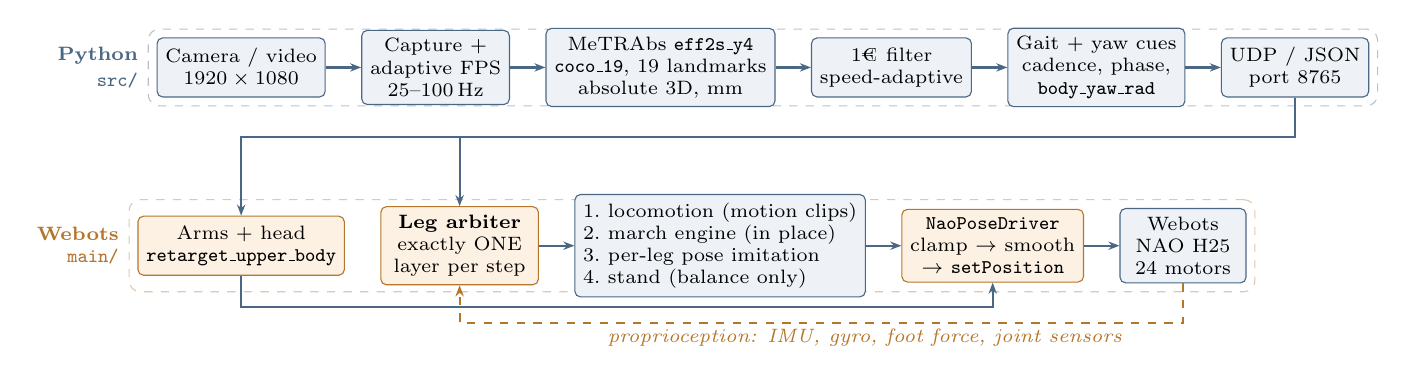
\begin{tikzpicture}[node distance=4.5mm]
  \node[blk, minimum width=18mm] (cam)  {Camera / video\\\scriptsize $1920\times1080$};
  \node[blk, right=of cam, minimum width=18mm] (cap) {Capture $+$\\adaptive FPS\\\scriptsize 25--100\,Hz};
  \node[blk, right=of cap, minimum width=24mm] (pose) {MeTRAbs \texttt{eff2s\_y4}\\\scriptsize \texttt{coco\_19}, 19 landmarks\\\scriptsize absolute 3D, mm};
  \node[blk, right=of pose, minimum width=18mm] (filt) {1\euro{} filter\\\scriptsize speed-adaptive};
  \node[blk, right=of filt, minimum width=18mm] (gait) {Gait $+$ yaw cues\\\scriptsize cadence, phase,\\\scriptsize \texttt{body\_yaw\_rad}};
  \node[blk, right=of gait, minimum width=17mm] (udp) {UDP / JSON\\\scriptsize port 8765};

  \draw[flow] (cam) -- (cap);   \draw[flow] (cap) -- (pose);
  \draw[flow] (pose) -- (filt); \draw[flow] (filt) -- (gait);
  \draw[flow] (gait) -- (udp);

  \node[acc, below=15mm of cam, minimum width=21mm] (upper) {Arms $+$ head\\\scriptsize \texttt{retarget\_upper\_body}};
  \node[acc, right=of upper, minimum width=20mm] (arb) {\textbf{Leg arbiter}\\\scriptsize exactly ONE\\\scriptsize layer per step};
  \node[blk, right=of arb, align=left, minimum width=29mm] (layers)
       {\scriptsize 1.\ locomotion (motion clips)\\
        \scriptsize 2.\ march engine (in place)\\
        \scriptsize 3.\ per-leg pose imitation\\
        \scriptsize 4.\ stand (balance only)};
  \node[acc, right=of layers, minimum width=23mm] (drv) {\texttt{NaoPoseDriver}\\\scriptsize clamp $\rightarrow$ smooth\\\scriptsize $\rightarrow$ \texttt{setPosition}};
  \node[blk, right=of drv, minimum width=16mm] (nao) {Webots\\NAO H25\\\scriptsize 24 motors};

  \draw[flow] (udp.south) -- ++(0,-5mm) -| (upper.north);
  \draw[flow] (udp.south) -- ++(0,-5mm) -| (arb.north);
  \draw[flow] (arb) -- (layers);
  \draw[flow] (layers) -- (drv);
  \draw[flow] (upper.south) -- ++(0,-4mm) -| (drv.south);
  \draw[flow] (drv) -- (nao);
  \draw[ret] (nao.south) -- ++(0,-5mm)
       -| node[lbl, accline, pos=0.22, below]
            {proprioception: IMU, gyro, foot force, joint sensors} (arb.south);

  \begin{scope}[on background layer]
    \node[draw=blkline!40, dashed, rounded corners, fit=(cam)(udp), inner sep=3pt,
          label={[font=\scriptsize\bfseries, blkline]left:\shortstack[r]{Python\\\texttt{src/}}}] {};
    \node[draw=accline!40, dashed, rounded corners, fit=(upper)(nao), inner sep=3pt,
          label={[font=\scriptsize\bfseries, accline]left:\shortstack[r]{Webots\\\texttt{main/}}}] {};
  \end{scope}
\end{tikzpicture}
\caption{End-to-end architecture. The Python side is a generic pose source; all NAO-specific
logic resides on the robot side. The dashed return path carries the robot's own
proprioception, the only available source of balance information.}
\label{fig:arch}
\end{figure*}

\textbf{Protocol.} One UDP JSON datagram is sent per processed frame to
\texttt{127.0.0.1:8765}. The payload is current state rather than a transaction, so a lost
packet is discarded rather than retransmitted behind newer data; the controller holds its last
pose if nothing arrives within $0.5$~s. The primary block carries 19 landmarks as
$[x, y, z, \text{visibility}]$ in millimetres in the camera frame. A second block carries
cadence, phase, stop state and \texttt{body\_yaw\_rad} as an angle rather than a turn intent,
so the controller can close a heading loop on it; its confidence is reported separately,
because the yaw estimate needs only shoulders and hips and survives the legs leaving frame. A
legacy joint-angle block is used only when no landmarks are present.

\textbf{World requirements.} Two settings are mandatory and committed in the world file.
\texttt{Nao.proto} tags its soles with the contact material \texttt{"NAO foot material"}, and
without a matching \texttt{ContactProperties} entry ($\mu = 8$, no bounce) the sole-floor pair
falls back to the Webots default. The feet then slide, the robot cannot load a single foot,
and the leg controller appears frozen because every command is absorbed by foot slip. This was
the most frequent cause of unresponsive legs during development. Second,
\texttt{basicTimeStep} must not exceed $20$~ms; the Webots default of $32$~ms is too coarse
for NAO leg control and destabilises the pre-balanced walk clips.

%%%%%%%%%%%%%%%%%%%%%%%%%%%%%%%%%%%%%%%%%%%%%%%%%%%%%%%%%%%%%%%%%%%%%%%%%%%%%%
\section{Perception}
%%%%%%%%%%%%%%%%%%%%%%%%%%%%%%%%%%%%%%%%%%%%%%%%%%%%%%%%%%%%%%%%%%%%%%%%%%%%%%

Frames are acquired through OpenCV~\cite{bradski2000opencv} at $1920\times1080$ with backend
fallbacks. A closed-loop controller adjusts the target rate between $25$ and $100$~FPS against
a $150$~ms latency budget on a 30-sample rolling mean, stepping down by $5$~FPS above the
budget and up by $5$~FPS below $0.65$ of it, the hysteresis preventing oscillation.

Pose estimation uses MeTRAbs \texttt{eff2s\_y4}~\cite{sarandi2021metrabs, abadi2016tensorflow}
with its built-in YOLOv4 detector~\cite{bochkovskiy2020yolov4}, emitting the \texttt{coco\_19}
skeleton~\cite{lin2014coco} as absolute metric coordinates. Joint names are read from the live
model at start-up and matched against canonical names through an alias table; a mismatch is a
hard start-up failure, since transposing two joints yields a robot that moves confidently and
incorrectly. An earlier iteration used MediaPipe BlazePose~\cite{bazarevsky2020blazepose},
whose normalised image coordinates and weak depth channel forced downstream code to reconstruct
3D from a frontal-projection assumption; MeTRAbs replaces that reconstruction with an exact
decomposition of a measured bone direction, at the cost of a GPU requirement and the loss of
per-landmark visibility and built-in temporal filtering.

\subsection{Tracked-box inference}

\texttt{detect\_poses} evaluates both the detector and the pose network at $75.9$~ms per frame,
of which the detector alone is $39.7$~ms. Supplying the previous frame's joints as the
detection box costs $36.2$~ms and returns bit-identical joints on a held pose.
Table~\ref{tab:detint} gives the resulting trade-off.

\begin{table}[H]
\centering
\caption{Detection-interval sweep: 90 frames, live moving subject, RTX~3090~Ti. Drift is
per-joint error relative to per-frame detection.}
\label{tab:detint}
\small
\begin{tabular}{@{}ccccc@{}}
\toprule
Interval & FPS & Median & p95 & Phantoms \\
\midrule
1 & 12.1 & n/a & n/a & n/a \\
\textbf{2} & \textbf{16.0} & \textbf{6.8\,mm} & \textbf{120\,mm} & \textbf{0} \\
3 & 17.7 & 6.8\,mm & 330\,mm & 0 \\
5 & 17.6 & 232\,mm & 536\,mm & 0 \\
\bottomrule
\end{tabular}
\end{table}

An interval of 2 buys $32\%$ throughput for millimetre-scale error; beyond 3 drift grows
rapidly while throughput does not. A continuity gate protects the schedule, since
\texttt{estimate\_poses} has no detector and will return a confident skeleton of an empty scene
given a stale box: any frame whose median per-joint displacement exceeds $300$~mm triggers a
full re-detection. The measured phantom-pose count was zero at every interval.

Because MeTRAbs reports only one detection-box score per person, a visibility proxy is
synthesised: $1.0$ well inside both box and image, decaying to $0.0$ within a $6\%$ edge margin
or outside the box. It measures framing rather than occlusion and is documented as such at
every consumer.

\subsection{Speed-adaptive smoothing}

A fixed-$\alpha$ exponential average cannot damp per-frame jitter without cost, since its group
delay of $(1-\alpha)/\alpha$ samples is independent of subject motion. At the measured rate of
$14.3$~FPS, $\alpha = 0.50$ costs $70$~ms, which is $47\%$ of the latency budget spent on the
keypoint channel alone and directly observable as robot lag. The 1\euro{}
filter~\cite{casiez2012oneeuro} instead makes the cutoff a function of speed, applied per axis
per landmark with a minimum cutoff of $1.0$~Hz and $\beta = 0.005$~Hz per mm/s. The scaling is
unit-dependent: a brisk limb moves at $1000$ to $2000$~mm/s, so $\beta$ opens the cutoff by $5$
to $10$~Hz, and with Nyquist at $7.2$~Hz that range separates smoothing from pass-through.

\subsection{Gait and heading cues}

The robot cannot walk by copying leg angles, so the lower body is distilled into a depth-free
gait command conveying intent. The primary signal is the knee-height difference normalised by a
smoothed body width,
\begin{equation}
s(t) = \big(y^{L}_{\text{knee}}(t) - y^{R}_{\text{knee}}(t)\big) \big/ w_{\text{body}}(t),
\label{eq:gaitsig}
\end{equation}
which is anti-phase between the knees, therefore large only when the legs alternate and
structurally immune to arm swing. Zero crossings give cadence, sign gives the raised knee,
amplitude gives vigour, and the normalisation makes it scale-invariant. Amplitude is measured
over $1.3$~s but crossings are counted over $3.0$~s: requiring two crossings in the shorter
window imposes a cadence floor of $0.385$~Hz, which is $2.6$ times the controller's minimum
request and held the marching state to $1.1\%$ of frames in recorded sessions.

NAO has no torso-yaw joint, so subject rotation must be imitated by stepping round, which
requires a heading angle. As the subject turns, the shoulder and hip lines shorten laterally
through foreshortening while their endpoints separate in depth, giving
\begin{equation}
\psi = \operatorname{atan2}\!\left(\Delta z,\; \Delta x\right), \quad
\Delta x = x_{\text{left}} - x_{\text{right}}.
\label{eq:yaw}
\end{equation}
Retaining the sign of $\Delta x$ extends the estimate from a quarter circle to the full circle:
beyond $90\degree$ the shoulders exchange sides in the image, and that sign change is the
front-back discriminator otherwise unavailable to one camera. The ordering follows the COCO
convention, in which a subject facing the camera is labelled with the anatomical left shoulder
on the image's right; measured on recorded runs the reverse ordering was negative on $67\%$ of
frames with both shoulders visible, $99\%$ of which also showed both ears.

Yaw robustness matters more than accuracy, because a noisy heading makes the controller request
turn clips in alternating directions, starving forward walking and tripping the locomotion
failure backoff. Three guards address this. Span gating compares the observed segment length
against a self-calibrated peak-hold reference, rejecting collapsed detections instead of
converting them into large angles. Shortest-arc smoothing ($\alpha = 0.18$) respects the
circular topology and averages shoulder and hip contributions as vectors. Jump de-weighting
halves the confidence of a frame disagreeing with the running estimate by more than $0.60$~rad
while still following it, so the estimator cannot latch. Replayed over the same sessions, turn
requests fell from $1438{+}53$ and $846{+}1206$ to $9{+}8$ and $11{+}15$, and the planner
remained in its standing state for $83$ to $86\%$ of frames.

%%%%%%%%%%%%%%%%%%%%%%%%%%%%%%%%%%%%%%%%%%%%%%%%%%%%%%%%%%%%%%%%%%%%%%%%%%%%%%
\section{Whole-Body Retargeting}
%%%%%%%%%%%%%%%%%%%%%%%%%%%%%%%%%%%%%%%%%%%%%%%%%%%%%%%%%%%%%%%%%%%%%%%%%%%%%%

NAO joint angles are defined relative to its own body, so with metric depth allowing the
subject to face any direction, each frame the retargeter builds an orthonormal torso-local
basis from the shoulder line and the hip-to-shoulder line:
\begin{align}
\mathbf{r} &= \mathrm{unit}\left(\mathbf{p}_{\text{Rsh}} - \mathbf{p}_{\text{Lsh}}\right), \nonumber\\
\mathbf{u}_0 &= \mathrm{unit}\left(\mathbf{p}_{\text{sh}} - \mathbf{p}_{\text{hip}}\right), \nonumber\\
\mathbf{u} &= \mathrm{unit}\left(\mathbf{u}_0 - (\mathbf{u}_0 \cdot \mathbf{r})\,\mathbf{r}\right),
\quad \mathbf{f} = \mathbf{r} \times \mathbf{u}.
\label{eq:basis}
\end{align}
Every bone vector is projected onto this basis before solving, so the recovered angles are
relative to the subject's own body rather than to the camera.

Each two-degree-of-freedom joint is then solved as two sequential rotations about fixed local
axes, a closed-form inverse of the chain the robot's joints implement. For a thigh at hip roll
$\varphi$ and hip pitch $\theta$, the unit bone direction is
$(\ell, u, f) = (\sin\varphi\cos\theta,\, -\cos\varphi\cos\theta,\, \sin\theta)$, with $\ell$
lateral, $u$ vertical and $f$ forward. All three components are measured directly, so the
inverse is exact:
\begin{align}
d = -u = \cos\varphi\cos\theta, \quad \varphi &= \operatorname{atan2}(\ell,\, d), \nonumber \\
\theta &= \pm \arccos\!\left(d / \cos\varphi\right),
\label{eq:inv}
\end{align}
with the sign of $\theta$ taken from $f$. The shank shares the hip roll and adds
\texttt{KneePitch} about the same axis, so the same solve on the knee-to-ankle vector yields
$\theta_{\text{hip}} + \theta_{\text{knee}}$; the sole is levelled by
$\texttt{AnklePitch} = -(\theta_{\text{hip}} + \theta_{\text{knee}})$ and
$\texttt{AnkleRoll} = -\varphi$. The same solve recovers the shoulder from the observed arm
direction. Segment lengths are measured in millimetres each frame and lightly smoothed; with no
foreshortening to correct, nothing must be learned online.

Foot-lift and crouch detection deliberately remain in camera-frame vertical, since ground
contact is a question of real-world verticality and resolving it in the torso frame would make
a forward lean register as a foot lift. Lift detection needs no floor model: the lower foot
defines the ground line and the other foot's rise above it is the lift. Subjects standing close
to a webcam are typically cropped at the shins, which made this read exactly zero, so the same
relative measure falls back to the knees, which are in frame whenever the hips are. Without a
visible ankle the knee bend is unobservable, so a lift then manifests as hip flexion, producing
a raised straight leg; this is the correct reading of the available information and is reported
as such in the status line.

%%%%%%%%%%%%%%%%%%%%%%%%%%%%%%%%%%%%%%%%%%%%%%%%%%%%%%%%%%%%%%%%%%%%%%%%%%%%%%
\section{Balance and Whole-Body Control}
%%%%%%%%%%%%%%%%%%%%%%%%%%%%%%%%%%%%%%%%%%%%%%%%%%%%%%%%%%%%%%%%%%%%%%%%%%%%%%

\subsection{Arbitration and the crouch family}

Exactly one layer commands the twelve leg joints on any simulation step, since concurrent
commanders contend and the robot falls. The four layers, in priority order, are locomotion
clips, the in-place march engine, per-leg pose imitation and standing balance; one
configuration constant selects the active subset, making bisection of a misbehaving
demonstration a one-line change.

The commanded posture is always $\mathrm{crouch}(u)$, defined by $\texttt{Hip} = -u$,
$\texttt{Knee} = +2u$ and $\texttt{Ankle} = -u$ so the three sum to zero, plus the human's
authority-weighted per-leg deviation from it. Because the NAO thigh ($100.0$~mm) and tibia
($102.9$~mm) agree within $3$~mm, this keeps the ankle beneath the hip, and therefore the
centre of mass over the foot, at any depth with the torso vertical and the soles flat. The
consequence is architectural: the symmetric component of the pose never leaves a stable family,
only asymmetric detail is gated, and a stationary subject produces zero deviation. It follows
that the squat limit of $40\degree$ hip and $80\degree$ knee is a joint-range constraint rather
than a stability one.

\subsection{Authority by symmetry}

Two distinct cases are conflated by ``the legs are at different angles'', and gating them
identically was incorrect. Mirror-symmetric poses, such as bilateral abduction into a wider
stance or equal bilateral flexion into a squat, leave the centre of mass unchanged by symmetry
and enlarge the support polygon; being safer than standing, they pass at full authority.
Antisymmetric poses, such as bilateral roll or one leg forward and one back, displace the
centre of mass. They are still followed at unity gain, but the robot shifts its pelvis to
render the pose holdable rather than attenuating it, under three bounds: the lean is capped at
$0.45$~rad, about $72$~mm of centre-of-mass travel; the antisymmetric channels are rate-limited
to $1.2$~rad/s, since a marching leg swing reproduced on two planted feet is a rocking
excitation; and once pelvis travel is exhausted the pose is scaled back, slewed to prevent
oscillation.

Stance width saturates at the ankle rather than the hip. \texttt{HipRoll} reaches $45.3\degree$
but \texttt{AnkleRoll} only $22.8\degree$, and the ankle is what levels the sole against hip
abduction. Refusing to exceed $22.8\degree$ proved too conservative, since recorded subjects
spread to $25\degree$ routinely, so a sole-tilt budget of $0.05$~rad is allocated, at which the
outer edge of a $76$~mm foot lifts about $4$~mm. At the original $0.15$~rad only the inner sole
corners contacted, and recorded logs show the robot standing on its foot edges immediately
before every lateral fall. The budget is enforced as a post-condition on the final commanded
angles with the hip yielding first, so when it binds, stance width yields and sole contact is
preserved. The result tracks the subject to about $30\degree$, saturating at $31.4\degree$ per
leg.

\subsection{Single-foot lift sequencing}

Raising a foot on a free-standing biped is three actions rather than one, and omitting the
first two is why a raised leg initially produced no visible response (Fig.~\ref{fig:liftfsm}).
The lean direction during LOAD is probed against the centre-of-mass model rather than
hard-coded, since an incorrect lean sign accelerates tipping. Three gates stand the robot down:
torso tilt beyond $0.40$~rad, low lower-body landmark confidence, and simultaneous absence of
both feet, which indicates a jump or tracking failure but never a step.

\begin{figure}[H]
\centering
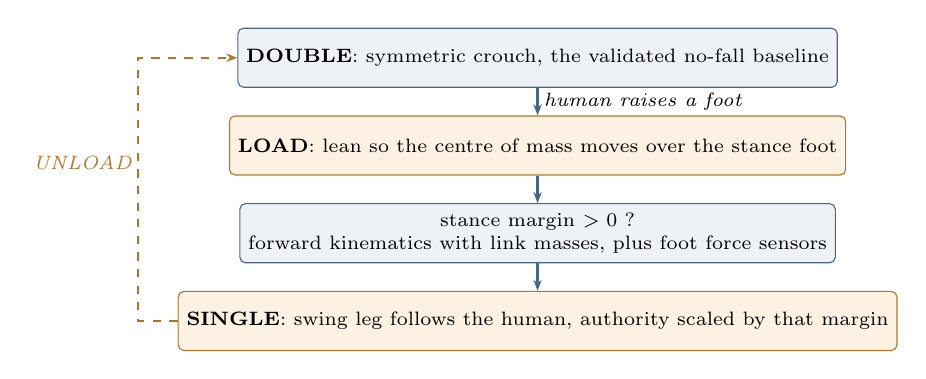
\begin{tikzpicture}[node distance=3.5mm]
  \node[blk, minimum width=52mm] (dbl)
       {\textbf{DOUBLE}: symmetric crouch, the validated no-fall baseline};
  \node[acc, below=of dbl, minimum width=52mm] (load)
       {\textbf{LOAD}: lean so the centre of mass moves over the stance foot};
  \node[blk, below=of load, minimum width=52mm] (gate)
       {stance margin $> 0$ ?\\\scriptsize forward kinematics with link masses,
        plus foot force sensors};
  \node[acc, below=of gate, minimum width=52mm] (sgl)
       {\textbf{SINGLE}: swing leg follows the human, authority scaled by that margin};
  \draw[flow] (dbl) -- node[lbl, right] {human raises a foot} (load);
  \draw[flow] (load) -- (gate);
  \draw[flow] (gate) -- (sgl);
  \draw[ret] (sgl.west) -- ++(-5mm,0)
       |- node[lbl, accline, pos=0.30, left] {UNLOAD} (dbl.west);
\end{tikzpicture}
\caption{Weight-transfer sequencer. Shift and lift are rate-limited blends in $[0,1]$, so there
are no discrete transitions and no state that can become stuck. UNLOAD is entered when the foot
is lowered, the margin is lost, or the torso tilts.}
\label{fig:liftfsm}
\end{figure}

The foot force sensors scale lift gain between $0.40$ and $1.0$ as the stance foot's load share
rises, confirming rather than vetoing. An earlier version vetoed outright, so a sensor
reporting a constant even split permanently prohibited stepping. By the time this gate
evaluates, the centre-of-mass model has already confirmed the transfer, and the tilt abort is
the real safety net.

\subsection{Centre-of-mass management}

Two terms move the pelvis on the same degree of freedom, hip $+c$ and ankle $-c$ bilaterally,
which translates the pelvis while keeping the soles flat. A feed-forward term asks whether the
commanded pose is statically holdable, computed from forward kinematics of the commanded
targets with no tilt term. A feedback term asks whether the robot is actually tipping, computed
from the measured posture and the IMU tilt with $0.12$~s of gyro lead. The driver computes the
feedback first and passes it into the lower-body controller, where the two are summed, clamped
once ($0.30$~rad pitch, $0.25$~rad roll) and rate-limited to $1$~rad/s. When the budget is
exhausted the feed-forward term yields, leaving feedback as the safety net. The two were
formerly independent, each with its own clamp, so two controllers answered every tilt in full;
their clamps summed to $0.55$~rad, about $85$~mm of travel against a margin budget of $40$ to
$60$~mm, and every fall in the logs carries that signature.

The model applies forward kinematics to the measured joint angles, places each link's local
centre of mass in a common frame using documented NAO link masses, and takes the mass-weighted
average $\mathbf{c} = M^{-1}\sum_i m_i \mathbf{T}_i \mathbf{c}_i$. Projecting it along gravity
and comparing with the support polygon yields a signed balance margin, with no Supervisor node
required. A fixed-sign PD controller on that error is fragile, since an incorrect sign makes
the feedback positive and accelerates tipping. The controller therefore searches: candidate
ankle and hip corrections are sampled on a golden-angle spiral of 24 points around the last
correction, the model predicts each resulting margin, and the best is applied. Because every
candidate is scored, the loop can only select corrections predicted to help, which confers
robustness to sign errors by construction.

The support polygon uses two contact tolerances. Whether a foot is grounded is judged loosely
against the other foot ($6$~mm), because the march knee bob shortens one leg by $3.2$~mm and
classifying that foot as airborne would report a negative margin for a robot standing squarely.
Which corners of a grounded foot carry load is judged tightly against that foot's own lowest
corner ($2$~mm), since a sole tilted by $0.05$~rad lifts its outer corner only $1.9$~mm.

%%%%%%%%%%%%%%%%%%%%%%%%%%%%%%%%%%%%%%%%%%%%%%%%%%%%%%%%%%%%%%%%%%%%%%%%%%%%%%
\section{Locomotion}
%%%%%%%%%%%%%%%%%%%%%%%%%%%%%%%%%%%%%%%%%%%%%%%%%%%%%%%%%%%%%%%%%%%%%%%%%%%%%%

The robot translates by playing Webots' pre-balanced NAO motion clips, tuned by Cyberbotics for
this robot~\cite{michel2004webots, gouaillier2009nao}. Synthesising an online gait for a
free-standing NAO is a research project in itself, and teleporting the base through a
Supervisor node destabilises the physics. Without clips on disk the controller falls back to
the march engine, which tracks cadence, phase and stop but marches in place.

\textbf{Preparation ramp.} Every walk and turn clip opens in a deep, sole-flat crouch of about
$0.51$~rad, while the controller stands at $u = 0.10$. Since playback commands the first
keyframe immediately with the velocity caps already lifted, direct handover demands $0.84$~rad
of knee travel in one $20$~ms step. The arbiter therefore reads the clip's first keyframe,
ramps the legs to it, and starts playback only once the measured joints have arrived. All
joints must arrive together: the knee travels $0.842$~rad, the hip $0.405$ and the ankle
$0.437$, and since sole attitude is their sum, a single flat rate drives that sum to
$0.405$~rad, eight times the tilt budget, and the support margin to $-0.064$~m. Scaling each
joint's rate by its share of the longest travel gives a sum of $0.0000$~rad and a margin of
$+0.0596$~m in the same $0.56$~s. The return is a ramp too, seeded from the posture the clip
left, since a clip ends in the same squat.

\textbf{Exit policy.} A clip boundary is a balanced double-support pose, so playing the whole
clip is the safe default, but that makes clip length the latency of stopping and imposes the
start-stop transient on every stride. That transient is $49\%$ of \texttt{Forwards.motion}'s
$2.60$~s, and during the closing settle the torso travels $17$~mm backward, which is why
chained clips measured $0.036$~m/s against a documented $0.10$~m/s. Three exits exist, in order
of preference: leaving a detectable gait cycle, stopping at a safe keyframe, and the tilt
abort. The second has a momentum component that is easy to miss, since stopping the legs does
not stop the robot: the capture point~\cite{pratt2006capture} lies $v/\omega$ ahead of the
centre of mass with $\omega \approx 5.9$~rad/s at this crouch, so $0.18$~m/s throws it $30$~mm
past the centre of mass against a $40$ to $60$~mm budget. Thirteen of the $46$ poses passing
the static test are moving that fast.

\textbf{Cyclic gait.} The clips are animations comprising squat, acceleration, stride,
deceleration and stand; the stride is satisfactory and the surrounding transient is the cost.
The middle of the long walk clip is a true limit cycle, with
$\max_j |q_j(4.23\,\mathrm{s}) - q_j(2.95\,\mathrm{s})| = 0.0000$~rad over all twelve leg
joints. The segment can therefore be rewound with \texttt{setTime()} without commanding joint
motion at the seam, making one clip a gait generator: a $1.28$~s stride advancing $0.093$~m,
giving $0.073$~m/s sustained. The schedule is derived from the clip's keyframes at run time rather than tabulated,
so it cannot diverge from the shipped files, and a non-cyclic clip is detected rather than
looped on assumption. The seam must be exact to one microradian, since it is a teleport
executed in one step with the caps lifted, and the cycle must translate the robot by at least
$0.02$~m, since looping a turn or side-step would rotate or drift it indefinitely. Cycling does
not lengthen the stride; it removes the transient between strides, reducing a $10$~s walk from
47 stand-squat cycles to one.

\textbf{Trimming the tail.} Leaving the cycle jumps into the clip's own deceleration, but that
tail is not uniformly deceleration. After $8.45$~s the clip commands no further travel and the
remaining $1.28$~s merely returns the legs to a standing posture, which the pose layer has to
undo the moment it regains them. Ending playback at the first certified keyframe past which no
travel remains cuts the worst-case stop from $3.73$ to $2.46$~s without ever stopping the robot
on momentum.

\textbf{Heading servo.} Open-loop turning does not converge, because clip and human turn by
different amounts and the error accumulates. The loop is closed on the robot's measured
heading, with the desired heading latched relative to where the subject was first observed and
the planner selecting a turn clip from the wrapped error each step. Two parameters determine
convergence. The planner refuses a clip that would overshoot: firing at $|e| = f n$ for nominal
turn $n$ leaves $|e - n| = |1 - 1/f|\,|e|$, which is at least $|e|$ for every $f \le 0.5$, so
the shipped value of exactly $0.5$ turned the robot from $+e$ to $-e$ indefinitely; at $0.65$
each turn reduces the error to at most $0.54$ of its previous value. The watchdog budget must
also derive from the clip's own duration without a ceiling, since \texttt{TurnLeft180} runs
$9.0$~s and the default $8.0$~s cap guaranteed an overrun.

\textbf{Aimed turning.} The overshoot rule above is correct for a clip played whole and wrong
for one that can be stopped part-way, and treating every clip as atomic made turning both slow
and coarse. The $40\degree$ clips spend roughly $60\%$ of their duration on their own start-stop
transient and so sustain only $13.8\degree$/s, against $20.7\degree$/s for the $180\degree$
clip; a $90\degree$ turn built from three of them pays that transient three times and settles
twice between. Since \texttt{safe\_exit\_times} already certifies the keyframes at which
playback may simply stop, and a stepping turn comes to rest at every footfall, pairing those
keyframes with the yaw the clip has delivered by each of them --- recovered by the same
stance-foot odometry used for translation --- yields a ladder of $104$ angles spaced at most
$16\degree$ apart. The controller re-evaluates the live heading error each step and stops at the
rung that minimises it, so the residual is bounded by half the spacing rather than by half a
clip. Two further rules follow: a rotation already running keeps its clip, since swapping
mid-turn costs a settle and a re-preparation; and the overshoot floor is retained for any clip
that cannot be stopped part-way, where it prevents a limit cycle in which a $60\degree$ clip
asked to correct $17\degree$ overshoots to $-43\degree$ and asks again.

\textbf{Freeze resistance.} A clip owns the whole body, so anything preventing it from
reporting completion would freeze the entire robot. A watchdog bounds suspension and retires
the offending clip, a failure backoff abandons clips after three bad attempts since repeated
falling is worse than never walking, and a settled-start check ensures clips start only from
an upright, calm robot. Separately, an exception in a control step is logged and the body
reclaimed rather than terminating the loop, which previously zeroed every motor velocity.

%%%%%%%%%%%%%%%%%%%%%%%%%%%%%%%%%%%%%%%%%%%%%%%%%%%%%%%%%%%%%%%%%%%%%%%%%%%%%%
\section{Sensing and Diagnosis}
%%%%%%%%%%%%%%%%%%%%%%%%%%%%%%%%%%%%%%%%%%%%%%%%%%%%%%%%%%%%%%%%%%%%%%%%%%%%%%

\subsection{InertialUnit axis masking}
\label{sec:imu}

\texttt{Nao.proto} mounts the inertial unit rolled $+90\degree$ about $x$ and declares
\texttt{yAxis FALSE}. The mount rotation is only an offset, absorbed by a learned tilt zero.
The axis mask is the defect: it is intended to disable the yaw output, and Webots implements it
by converting the sensor attitude to axis-angle, zeroing the world-$z$ component of the axis,
and re-deriving roll, pitch and yaw. On an upright sensor this is harmless; on one rolled
$90\degree$ it corrupts axes it was not asked to modify. Composing
$R^{\text{sensor}}_{\text{world}} = R_{\text{torso}} R_x(\pi/2)$ and applying the Webots ENU
decomposition through the zeroing predicts Table~\ref{tab:imupath}.

\begin{table}[H]
\centering
\caption{Predicted \texttt{InertialUnit} output under axis masking. All three rows are
confirmed by the recorded logs.}
\label{tab:imupath}
\small
\begin{tabular}{@{}lccc@{}}
\toprule
Torso motion & Rep.\ roll & Rep.\ pitch & Rep.\ yaw \\
\midrule
pitch forward $b$ & $0$ & $\mathbf{b/2}$ & $\mathbf{b/2}$ \\
rotate by $\psi$ & $0$ & $\boldsymbol{\psi/2}$ & $\psi/2$ \\
roll right $b$ & $\mathbf{b}$ & $0$ & $0$ \\
\bottomrule
\end{tabular}
\end{table}

The pitch channel therefore reports half the true pitch and is indistinguishable from a body
rotation, while the yaw channel is not a heading but a copy of that half-pitch. Both
predictions hold across all sessions: over 41 logs the reported yaw tracks the raw reported
pitch at $r \ge 0.994$ with slope $\approx 1.0$, and a regression of reported pitch against the
torso pitch implied by the loaded foot's forward kinematics has slope $+0.48$, roll being
unaffected at $+0.98$. The correct compensation is to double the pitch on input, and a scale
constant exists for this; it ships at $1.0$ deliberately, because under-correction is sluggish
but stable whereas over-correction produces a fall. Since both the IMU yaw axis and the gyro
$z$ axis are disabled, no inertial sensor observes robot rotation, so the heading loop reads
the orientation matrix from the Supervisor interface instead.

\subsection{Gravity as an independent witness}
\label{sec:acc}

The accelerometer appears preferable in principle, with three enabled axes and gravity as an
absolute reference requiring no learned zero, and its derived roll matches the inertial unit to
four decimals on a stationary robot. Controlling from it nonetheless destabilises the system,
because an accelerometer measures gravity plus the robot's own acceleration and so feeds a
second derivative back as a position: the loop shifts the pelvis, the torso accelerates
laterally, the accelerometer reports that as tilt, and the loop shifts further. Within one
recorded session with no subject present, seven episodes using gravity fell within
approximately $2$~s each, while three using the inertial unit stood for $40$~s and then
$298$~s. The streak was ended by an automatic cross-check rather than by intervention: the roll
disagreement between sources latched and the accelerometer path disabled itself. That path
therefore ships disabled, and enabling it requires integrating the gyro for fast attitude with
gravity correcting only slow drift. Gravity is still logged every step, since it is the only
independent measurement of the half-scale pitch.

\subsection{Automated log analysis}

The significant failures in this project are statistical, such as a head pinned for $40\%$ of
frames or a support margin negative for $80\%$ of a run, and none is apparent from watching the
robot. An analyser of approximately $1{,}100$ lines reads each run's trajectory CSV and emits a
severity-ranked list of findings. Each of its twenty checks corresponds to a defect that
previously shipped, covering joint saturation, tracking error, immobile legs, support margin,
sole contact, concurrent commanders, falls, pelvis-shifter double clamping, tilt-sign
consistency, attitude-source regression, locomotion chain health, gait-cycle integrity and walk
speed.

%%%%%%%%%%%%%%%%%%%%%%%%%%%%%%%%%%%%%%%%%%%%%%%%%%%%%%%%%%%%%%%%%%%%%%%%%%%%%%
\section{Results}
%%%%%%%%%%%%%%%%%%%%%%%%%%%%%%%%%%%%%%%%%%%%%%%%%%%%%%%%%%%%%%%%%%%%%%%%%%%%%%

Table~\ref{tab:coverage} summarises the achieved imitation behaviour. The pattern is
consistent: joint range limits the symmetric motions, and the centre-of-mass model limits the
asymmetric ones.

\begin{table}[H]
\centering
\caption{Achieved imitation behaviour and its binding constraint.}
\label{tab:coverage}
\small
\begin{tabular}{@{}p{1.5cm}p{2.5cm}p{2.5cm}@{}}
\toprule
Human motion & Robot response & Limited by \\
\midrule
Arms, head & shoulder pitch and roll, elbow, head yaw and pitch & joint range \\
Squat & unity gain to $40\degree$ hip, $80\degree$ knee & knee range, not balance \\
Spread legs & unity gain to $30\degree$, saturating at $31.4\degree$ & ankle roll plus a $0.05$\,rad tilt budget \\
Lean, split stance & unity gain with pelvis shift & lean cap, then pelvis travel \\
Raise one leg & weight shifts, then full lift & centre-of-mass margin \\
Walk, march & translation via clips, else in place & clip availability, cue confidence \\
Turn & steps round the full circle & clip granularity \\
\bottomrule
\end{tabular}
\end{table}

\subsection{Perception timing}

Timings are from the target workstation (RTX~3090~Ti and RTX~3070, Python~3.12, Webots
\texttt{basicTimeStep} $20$~ms). Per-frame inference costs $75.9$~ms when the person detector
runs and $36.2$~ms on a tracked box, so at \texttt{detect\_interval}${}=2$ the mix averages
$\approx 56$~ms. Measured over $31{,}243$ consecutively recorded frames with a subject in
shot, the whole perception loop closes in $63$~ms at the median and $95$~ms at the 90th
percentile, i.e.\ $16.0$~FPS sustained. Inference is therefore essentially the entire budget:
the gait cue costs $0.030$~ms, the action cue $0.011$~ms, the 1\euro{} filter $0.022$~ms per
axis, the arbiter $0.002$~ms and a UDP round trip $0.005$~ms, together under $0.1$~ms. One
caveat for anyone repeating this: a frame containing no person returns in $42$~ms because the
pose network is skipped, so benchmarking on blank input understates the cost by about a
quarter.

Summing independently measured stages gives $\approx 121$~ms from camera exposure to motor
command for the arm and head channel: one $63$~ms frame period, up to one $20$~ms control step
of quantisation, and $38$~ms of residual lag in the arm filter, whose time-constant-plus-lead
formulation replaced a frame-rate-clocked exponential filter costing $108$~ms. This sits within
the $150$~ms requirement at the median but not at the 90th percentile. It remains a sum of
parts rather than a single stopwatch reading, because the controller logs its own control-step
counter rather than the pipeline's frame index; adding that one field would make the
end-to-end figure directly measurable and is the most valuable instrumentation still missing.

\subsection{Locomotion}

Table~\ref{tab:locomotion} reports the locomotion figures, all derived from the shipped clips'
own keyframes through the forward-kinematic mass model rather than from a tabulated
specification.

\begin{table}[H]
\centering
\caption{Locomotion, measured from clip kinematics.}
\label{tab:locomotion}
\small
\begin{tabular}{@{}p{3.9cm}p{3.2cm}@{}}
\toprule
Quantity & Measured \\
\midrule
Sustained walk speed, cyclic & $0.073$\,m/s \\
Walk speed, chained clips & $0.036$\,m/s \\
Stride period, advance & $1.28$\,s, $0.093$\,m \\
Limit-cycle seam error & $0.0000$\,rad (12 joints) \\
Peak commanded joint speed & $83.5\%$ of rated \\
Stop latency, cyclic exit & $2.46$\,s (was $3.73$) \\
Turn rate, aimed $180\degree$ clip & $20.7\degree$/s \\
Turn rate, $40\degree$ clips chained & $13.8\degree$/s \\
Turn $90\degree$ & $4.6$\,s, one clip, $1.1\degree$ residual \\
Turn $180\degree$ & $8.5$\,s, one clip, $3.9\degree$ residual \\
Smallest served heading error & $21\degree$ (was $26\degree$) \\
\bottomrule
\end{tabular}
\end{table}

Two results deserve comment. First, walking speed is hardware-bound, not tuning-bound: across
the clip's $2{,}376$ joint-intervals nothing exceeds the declared motor maximum, but the peak
reaches $83.5\%$ of it, so the clip cannot be retimed faster without commanding speeds the
motors cannot follow and desynchronising a dynamically balanced gait. Second, stop latency
fell from $3.73$ to $2.46$~s once the clip's closing $1.28$~s was identified as a return to
standing posture that commands no travel and that the pose layer must undo in any case; the
deceleration proper occupies only $1.18$~s of the $2.46$~s tail.

Aimed turning replaced clip chaining. Pairing each certified stopping keyframe with the yaw
the clip has delivered by then converts \texttt{TurnLeft180} into a ladder of $104$ reachable
angles spaced at most $16\degree$ apart, so a single clip stopped at the nearest rung bounds
the residual heading error at $8\degree$, against $20\degree$ for playing the $40\degree$ clip
whole. Replayed over eleven target headings, aimed turning reduced total time from $88.2$ to
$51.5$~s, clips played from $24$ to $11$, and mean residual error from $21.6\degree$ to
$3.9\degree$.

\subsection{Session logs}

Two instrumented sessions were recorded on 18~September, both at a real-time factor of $0.983$
($20.3$~ms of wall clock per $20$~ms simulation step). The first, $191$~s with a subject
tracked throughout, is the system behaving as designed: a motion clip owned the legs for
$54.0\%$ of tracked steps, and during confident marching that rose to $84.8\%$, with the
planner selecting a walk clip in $55.9\%$ of marching steps and a turn clip in $40.7\%$. Torso
tilt stayed small (median $|\mathrm{roll}|$ $0.005$~rad, 99th percentile $0.087$) and the
fore-aft support margin was negative in $2.0\%$ of steps.

The second session exposed a defect that no per-frame metric would have surfaced, and it is the
most consequential finding in the logs. At simulation time $21.1$~s the controller dropped all
eleven clips for the remainder of the run. The cause is a session-wide kill switch: three
consecutive failures retire locomotion entirely, and here a single preparation ramp toward
\texttt{forward} failed to reach the clip's opening stance three times in succession, spending
$7.94$~s in preparation before the third timeout disabled the layer. The run continued for a
further $2.5$~hours --- still in progress when this analysis was taken --- during which
$99.8\%$ of control steps executed with locomotion switched off and not one clip played. That
period is therefore not evidence about locomotion at all. It also illustrates a second problem
worth separating from the first: a subject was tracked in only $76$~s of that run, so the vast
majority of the record is an unattended robot standing still, and session length is a poor
proxy for evidence.

Two design consequences follow from the kill switch. The backoff counts failures over a whole
session with no decay, so three unlucky ramps minutes apart are indistinguishable from a
genuinely broken clip set; and because each failure calls the abandon path, which clears the
cumulative ramp clock, the $3.5$~s total-ramp ceiling intended to bound exactly this case can
never accumulate across attempts. Both are recorded as open items.

\subsection{The two-witness locomotion trigger}

The action classifier commits to walking only once the pelvis has travelled $80$~mm within
$0.8$~s, a threshold calibrated against one subject. A subject marching in place, or walking at
$0.07$ to $0.10$~m/s, does not satisfy it and is reported as idle, whereupon the planner
formerly returned an explicit stand without consulting the gait cue. The legs then fell through
to per-leg pose imitation of a walking human, which is neither balanced nor intended, and is
the mechanism behind the reported wobbling and falls. Replayed over the recorded session the
gait cue observed the legs cycling for $59$~s while the planner answered ``standing still'' for
$75\%$ of it.

Treating the two cues as independent witnesses to one question --- either the pelvis travels or
the legs cycle --- and letting the verdicts a cycling pair of legs contradicts yield to a
confident march raised coverage of marching intervals by clip-driven walking from $12.5\%$ to
$83\%$ on the 17~September session and from $30\%$ to $87\%$ on the 18~September session, while
posture clips fired during marching fell from $6.1\%$ to $0.4\%$ and false walking on frames
where the subject was demonstrably still remained at $0.0\%$. Walk intervals long enough to
reach the clip's stride loop rose from $6$ to $24$. The verdict for an unobserved subject is
deliberately exempt, since a gait cue retaining warm evidence would otherwise walk the robot at
a human who has left the frame.

\subsection{Implementation}

The implementation is $28{,}496$ lines of Python: $9{,}535$ of tests, $8{,}023$ of robot-side
mathematics, $4{,}176$ of pipeline, $3{,}864$ of Webots controllers and $2{,}889$ of tooling.
Every robot-side library is simulator-independent, so the control stack is testable without a
Webots installation. The suite covers the leg solve as a round trip, self-calibration and
cropped-feet lift detection, the step sequence and every safety gate, clip discovery, the
overshoot guard and the turn ladder, the centre-of-mass model and its spiral search, and a
re-derivation of the IMU tilt signs from the sensor mounting that prevents silent regression.
The integration suite exercises the real controller against a mocked Webots over real UDP,
including leg arbitration, motion hand-off and freeze resistance. At the time of writing
\texttt{pytest} collects and passes $575$ tests in $214$~s, with no failures or skips; the
cyclic-clip exit defect reported in an earlier revision has been resolved.

%%%%%%%%%%%%%%%%%%%%%%%%%%%%%%%%%%%%%%%%%%%%%%%%%%%%%%%%%%%%%%%%%%%%%%%%%%%%%%
\section{Limitations and Conclusions}
%%%%%%%%%%%%%%%%%%%%%%%%%%%%%%%%%%%%%%%%%%%%%%%%%%%%%%%%%%%%%%%%%%%%%%%%%%%%%%

\texttt{ElbowYaw} and \texttt{WristYaw} remain at rest, so forearm twist is not imitated;
recovering it requires hand landmarks \texttt{coco\_19} does not provide. Two defects found in
the session logs are open. The locomotion backoff retires all clips after three failures
counted over an entire session with no decay, so three unlucky preparation ramps minutes apart
are indistinguishable from a broken clip set; it disabled locomotion $21$~s into a
$8{,}077$~s run. The cumulative ramp ceiling intended to bound that case is cleared by the
abandon path on every failure and therefore never accumulates. Both need a decaying counter and
a clock that survives the abandon.

Walking speed is now bounded by the robot rather than the software: the shipped clip peaks at
$83.5\%$ of rated motor speed, so $0.073$~m/s cannot be improved by retiming. The turn clips
run at only $52\%$ and do have headroom, but retiming a dynamically balanced clip cannot be
validated by the quasi-static certifier, which already rejects the shipped clips, and so needs
live testing. Removing the quantisation altogether wants an online gait generator or a learned
policy~\cite{ze2025twist}; the heading servo already accepts a continuous action.

End-to-end latency is still a sum of separately measured stages rather than one measurement,
because the controller logs its own step counter instead of the pipeline's frame index. Two
further items warrant a check on the target machine: the torso-yaw sign convention against real
MeTRAbs output, and whether the IMU pitch scale can be raised toward the analytically correct
$2.0$. The accelerometer path wants a complementary or Kalman filter fusing gyro integration
with gravity. Finally, the action classifier's walk witnesses remain absolute speeds fitted to
one subject; expressing them relative to the subject's own leg length and a noise floor learned
at session start would remove the recalibration the two-witness trigger currently compensates
for. A per-joint error study against fixed reference motions would convert the
imitation-fidelity requirement from a target into a measurement; the logs and tooling exist.

A simulated humanoid can be teleoperated convincingly from one RGB camera, provided the
retargeted pose is treated as a request rather than a command. Three structural decisions
carried this project: retargeting in a torso-local basis, making the mapping invariant to
subject heading; enforcing that exactly one control layer owns the leg joints on any step; and
granting authority by whether a pose displaces the centre of mass, so mirror-symmetric motions
pass at full fidelity while displacing motions receive a compensating pelvis shift under
explicit bounds. The project's defects share a common character: the playback confirmation
defect, the double-clamped pelvis shift, the axis-masking artefact, the force-sensor veto and
the non-convergent overshoot fraction were all silent, with the robot continuing to behave
plausibly while a stated invariant was violated. None was found by observation. All were found
by stating the invariant the code claimed and then measuring, across whole recorded sessions,
whether it held.

%%%%%%%%%%%%%%%%%%%%%%%%%%%%%%%%%%%%%%%%%%%%%%%%%%%%%%%%%%%%%%%%%%%%%%%%%%%%%%
\section*{Acknowledgments}
%%%%%%%%%%%%%%%%%%%%%%%%%%%%%%%%%%%%%%%%%%%%%%%%%%%%%%%%%%%%%%%%%%%%%%%%%%%%%%

The authors thank M.Sc.~Severin Stahl (THM, Campus Friedberg, IEM) for supervising the project
and for guidance on scope, requirements and evaluation methodology. This work was carried out
as Group~C's project for the CSPM 2026S course, and was supported by the Department of
Information Technology, Electrical Engineering and Mechatronics at THM University of Applied
Sciences. The authors declare no conflicts of interest.

% =============================================================================
% NOTE TO THE AUTHORS: the contributions below are derived from the repository's
% commit history and module ownership. Please review and adjust before submission;
% only the two committing authors' roles are verifiable from the repository.
% =============================================================================
\textbf{Author contributions.} Tarik Billa designed the system architecture and process split
and implemented the perception pipeline, retargeting mathematics, leg-control arbiter, balance
and locomotion layers, and log-analysis tooling. Salih Keceli contributed to the Webots world
and robot configuration, simulation integration, and testing and validation of the control
stack. Niti Shivang Trivedi, Shantanu Shende, Sai Radhika Mitta and Amreen Fatima contributed
to requirements analysis, experiment design and session capture, evaluation of tracking and
gait-cue behaviour, and documentation. All authors reviewed and approved the final report.

\textbf{Data availability.} Source code, configuration, the Webots world, the test suite and
the analysis tooling are available in the project repository,
\href{https://github.com/tarikbilla/Pose-Imitation-of-Human-Motion-by-a-Simulated-Humanoid-Robot}%
{Pose Imitation of Human Motion by a Simulated Humanoid Robot}.
Recorded trajectory logs and demonstration videos are available on request. The MeTRAbs
pretrained weights carry a non-commercial-use training-data licence; the code itself is MIT.

\printbibliography[title={References}]

\end{document}
